\documentclass[11pt,compress,t,notes=noshow, aspectratio=169, xcolor=table]{beamer}

\usepackage{../../style/lmu-lecture}
% Defines macros and environments
% This file is included in slides and exercises

% Rarely used fontstyle for R packages, used only in 
% - forests/slides-forests-benchmark.tex
% - exercises/single-exercises/methods_l_1.Rnw
% - slides/cart/attic/slides_extra_trees.Rnw
\newcommand{\pkg}[1]{{\fontseries{b}\selectfont #1}}

% Spacing helpers, used often (mostly in exercises for \dlz)
\newcommand{\lz}{\vspace{0.5cm}} % vertical space (used often in slides)
\newcommand{\dlz}{\vspace{1cm}}  % double vertical space (used often in exercises, never in slides)
\newcommand{\oneliner}[1] % Oneliner for important statements, used e.g. in iml, algods
{\begin{block}{}\begin{center}\begin{Large}#1\end{Large}\end{center}\end{block}}

% Don't know if this is used or needed, remove?
% textcolor that works in mathmode
% https://tex.stackexchange.com/a/261480
% Used e.g. in forests/slides-forests-bagging.tex
% [...] \textcolor{blue}{\tfrac{1}{M}\sum^M_{m} [...]
% \makeatletter
% \renewcommand*{\@textcolor}[3]{%
%   \protect\leavevmode
%   \begingroup
%     \color#1{#2}#3%
%   \endgroup
% }
% \makeatother

\newcommand{\open}{}
\newcommand{\close}{}

\title{Interpretable Machine Learning}
% \author{LMU}
%\institute{\href{https://compstat-lmu.github.io/lecture_iml/}{compstat-lmu.github.io/lecture\_iml}}
\date{}

\begin{document}

\newcommand{\titlefigure}{figure/open_blackbox}
\newcommand{\learninggoals}{
\item What are additive decomposition of prediction functions?
\item Why are they useful?
\item How do we obtain them?}

\lecturechapter{Additive Decomposition}
\lecture{Interpretable Machine Learning}

\begin{frame}{Functional Decomposition
%\\
%\citebutton{Sobol (1993)}{http://www.andreasaltelli.eu/file/repository/sobol1993.pdf}
% \citebutton{Sobol (2003)}{https://doi.org/10.1016/S0951-8320(02)00229-6}
%\citebutton{Li et al. (2001)}{https://doi.org/10.1021/jp010450t}
\citebutton{Li and Rabitz (2011)}{https://doi.org/10.1007/s10910-011-9898-0}
\citebutton{Chastaing et al. (2012)}{https://doi.org/10.1214/12-EJS749}
}

%\textbf{High-Dimensional Model Representation (HDMR):} 
For interpretation purposes, one might be interested in decomposing a square-integrable function $\fh: \mathbb{R}^p \mapsto \mathbb{R}$ into sum of components of different dimensions w.r.t. inputs $x_1, \ldots, x_p$: %
\begin{equation*}
\begin{split}
\fh(\xv) =  %g_{\open \emptyset \close} +
\textstyle\sum_{S \subseteq \{1,\ldots,p\}} g_{S}(\xv_S) = \; & g_{\open \emptyset \close} + g_{\open 1 \close}(x_1) + g_{\open 2 \close}(x_2) + \dots + g_{\open p \close}(x_p) + \\
& g_{\open 1, 2 \close}(x_1, x_2) + \dots + g_{\open p-1, p \close}(x_{p-1}, x_p) + \dots + \\
& g_{\open 1,\ldots,p \close}(x_1, \ldots, x_p)
\end{split}
\end{equation*}
%\vspace{-5pt}%\pause
where 
\begin{itemize}
\item $g_{\open \emptyset \close} \hat = $ Constant mean (intercept) %$\mathbb{E}_X (\fh(\xv)) $
\item $g_{\open j \close} \hat = $ first-order or main effect of $j$-th feature alone on $\fh(\xv)$
%\item Bivariate terms $g_{\open j, k \close} \hat = $ second-order effect of features $j$ and $k$ w.r.t. $\fh(\xv)$%, etc.
\item $g_{S}(\xv_S) \hat = $ $|S|$-order effect, depends \textbf{only} on features in $S$ %$x_j$ for all $j \in S$
\end{itemize}
\lz
\textbf{N.B.:} %Further constraints are required to obtain an unique and optimal solution for the components
A unique solution for the components only exists under certain assumptions
%and constraints
%independent inputs and a \textit{vanishing condition}
%$$\mathbb{E}_{X_j} (g_{S}(\xv_S)) = \int g_{S}(\xv_S) d \mathbb{P}(x_j) = 0, \forall j \in S, \forall S \subseteq \{1, \ldots, p\}$$
%Without further constraints on components, there is no unique solution.
%\end{itemize}

%High-Dimensional Model Representation (HDMR)
%Functional ANOVA decomposition
%Sobol-Hoeffding decomposition
\end{frame}

\begin{frame}{Functional Decomposition -- Assumptions}
For independent inputs, the \textit{vanishing condition} is required to obtain a unique solution:
$$\mathbb{E}_{X_j} (g_{S}(\xv_S)) = \int g_{S}(\xv_S) d \mathbb{P}(x_j) = 0, \forall j \in S, \forall S \subseteq \{1, \ldots, p\}$$

\pause 

Vanishing condition has the following implications:

\begin{itemize}
    \item Marginalizing out $x_j, \forall j \in S$ for component $g_S(\xv_S)$ yields a constant 0\\
    %As we integrate out the marginal effect of $x_j, \forall j \in S$ on component $g_S(\xv_S)$ is zero (vanishes)\\
    $\leadsto$ Makes sure that component $g_S(\xv_S)$ does not contain effects of $x_j, \forall j \in S$
    %For $|S| = 1$ this is equivalent to mean-centering the component $g_S(\xv_S)$. For $|S| > 1$
    \item Components are orthogonal (i.e., mutually independent and uncorrelated):
    $$\mathbb{E}_{X} (g_{V}(\xv_V) g_{S}(\xv_S)) = 0, \forall V \neq S$$
    \item Variance can be decomposed:
$ Var[\fh(\xv)] =  \textstyle\sum_{S \subseteq \{1,\ldots,p\}}  Var\left[ g_{S}(\xv_S)\right]$
\end{itemize}

\pause 

\textbf{N.B.:} For dependent inputs, \citebutton{Hooker (2007)}{http://www.tandfonline.com/doi/abs/10.1198/106186007X237892} showed the existence of a unique solution for the components under a ``relaxed vanishing condition'' which leads to a ``hierarchical orthogonality''
$$\mathbb{E}_{X} (g_{V}(\xv_V) g_{S}(\xv_S)) = 0, \forall V \subset S$$
$\leadsto$ Only components are orthogonal where features involved in $g_{V}(\xv_V)$ also appear in $g_{S}(\xv_S)$
%Only components where all features involved in one component $g_{V}(\xv_V)$ also appear in the other component $g_{S}(\xv_S)$ are orthogonal
\end{frame}

\begin{frame}{Functional Decomposition -- Example}
\textbf{Example:} $\fh(\xv) = 2 + x_1^2 - x_2^2 + x_1 \cdot x_2$ (e.g., if $x_1 = 5$ and $x_2 = 10$ $\Rightarrow$ $\fh(\xv) = -23$)

\begin{itemize}
    \item Computation of components using feature values $x_1 = x_2 = (-10, -9, \ldots, 10)^\top$ gives:
    \begin{columns}[c, totalwidth=\linewidth]
    \begin{column}{0.75\textwidth}
        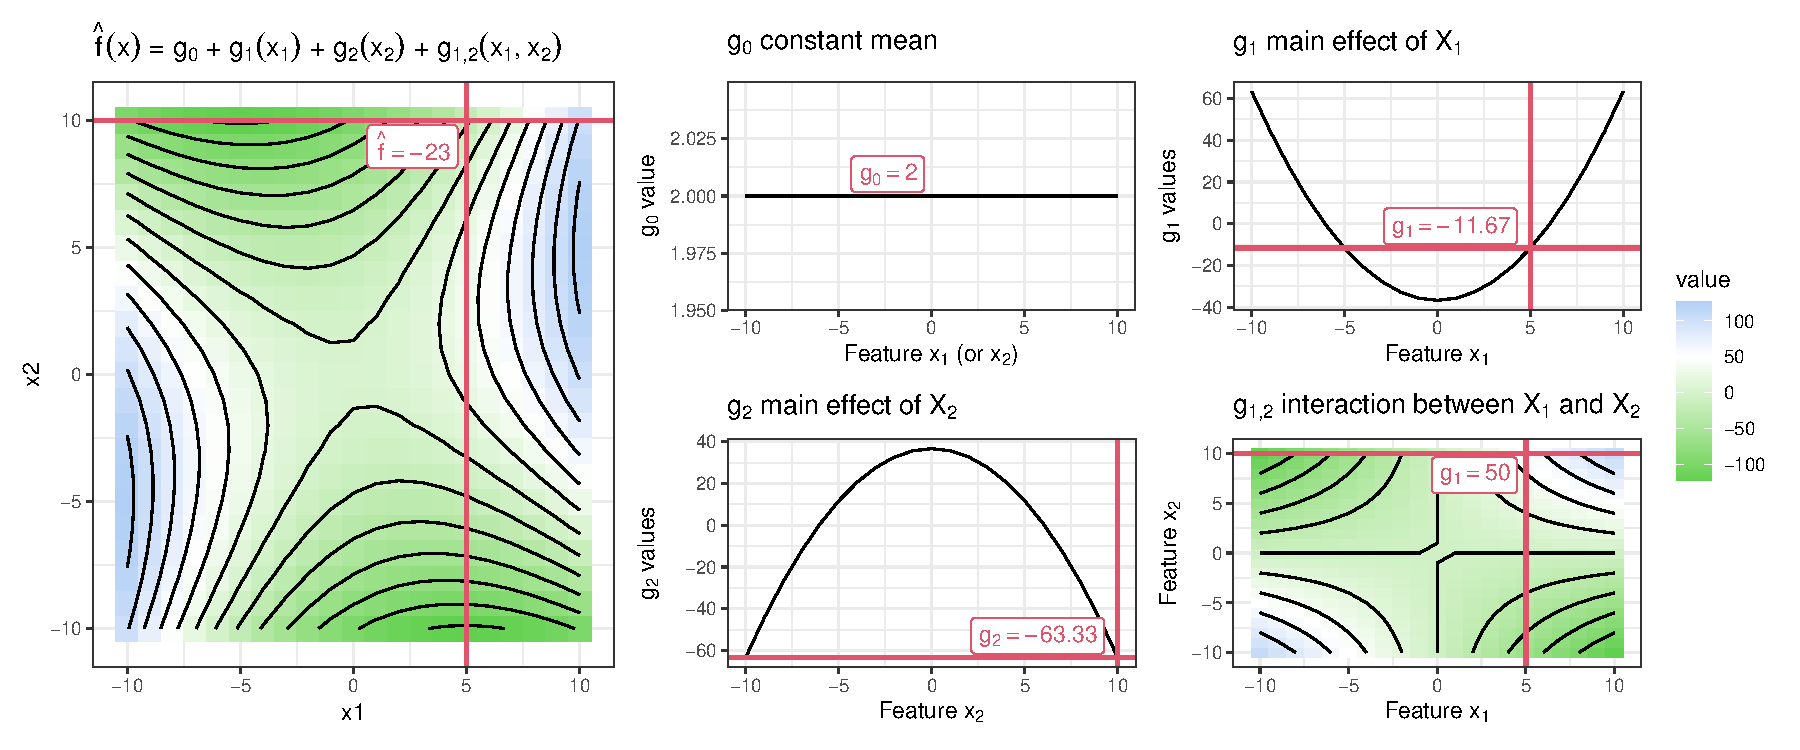
\includegraphics[width = \textwidth]{figure/decomposition}
    \end{column}
    \begin{column}{0.25\textwidth}
    For $x_1 = 5$ and $x_2 = 10$:\\
    \begin{itemize}
        \item $g_{\open \emptyset \close} = 2$
        \item $g_{\open 1 \close}(x_1) = -9.67$
        \item $g_{\open 2 \close}(x_2) = -65.33$
        \item $g_{\open 1,2 \close}(x_1, x_2) = 50$
        \item[$\Rightarrow$] $\fh(\xv) = -23$
    \end{itemize}
    \end{column}
    \end{columns}
\pause
    \item Vanishing condition means:
    \begin{itemize}
        \item $g_1$ and $g_2$ are mean-centered w.r.t. marginal distribution of $x_1$ and $x_2$
        \item Integral of $g_{1,2}$ over marginal distribution $x_1$ (or $x_2$) is always 0.
        %, i.e., for each slice at $x_1$ (and $x_2$), the integral of $g_{1,2}$ 
    \end{itemize}
\end{itemize} 
\end{frame}


% \begin{frame}{Functional Decomposition}

% Desirable properties of additive decomposition:

% \begin{itemize}
% \item Zero-means property (all components are centered): %\\
% $\mathbb{E}_{X_j} (g_{S}(\xv_S)) = 0, \forall S \neq \emptyset, j \in S$
% %$\mathbb{E}_{X_S} (g_{S}(\xv_S)) = 0, \forall S \neq \emptyset$ 
% % taken from 10.1007/s10910-011-9898-0 and 10.1137/130936233 (Q: Does this hold for arbitary distributions?) if not 
% % 
% \item Orthogonality (components are independent): %\\
% $\mathbb{E}_{X} (g_{V}(\xv_V) g_{S}(\xv_S)) = 0, \forall V \neq S$ 
% \item Variance decomposition:
% $ Var[\fh(\xv)] =  \textstyle\sum_{S \subseteq \{1,\ldots,p\}}  Var\left[ g_{S}(\xv_S)\right]$\\
% $\leadsto$ Only possible under orthogonality of components and if features are independent
% %effect terms of increasing order 
% %HDMR decomposes model into sum of effect terms of increasing order:
% % \begin{align*}
% % \fh(\xv) &= g_{\open \emptyset \close} + g_{\open 1 \close}(x_1) + g_{\open 2 \close}(x_2) + \;\dots\; + g_{\open 1, 2 \close}(x_1, x_2) \\
% % &\phantom{{}={}} + \;\dots\; + g_{\open 1,\ldots,p \close}(x_1, \ldots,x_p)
% % \end{align*}
% %\item Features need to be independent to make HDMR unique
% \end{itemize}

% \pause

% Different ways to compute the components exist, e.g.: % (with slightly different constraints / properties)
% 		\begin{itemize}
% 			\item %Recursive expectations (via partial dependence functions) \\
% 			Functional ANOVA decomposition for \textbf{independent features} \citebutton{Hooker (2004)}{http://portal.acm.org/citation.cfm?doid=1014052.1014122} \\
% 			$\leadsto$ By recursive expectations of partial dependence functions\\
% 			$\leadsto$ Satisfies all desirable properties
% 			% Often defined only for uniform distribution of x but Owen says it also applies to any distribution e.g. in 10.1137/130936233
% 			\item Generalized functional ANOVA decomposition for \textbf{dependent features} \citebutton{Hooker (2007)}{http://www.tandfonline.com/doi/abs/10.1198/106186007X237892} \\
% 			$\leadsto$ By minimizing squared error and relaxing the orthogonality property
% 			% https://epubs.siam.org/doi/abs/10.1137/16M1097717
% 			% Hierarchical orthogonality where $\mathbb{E}_{X} (g_{V}(\xv_V) g_{S}(\xv_S)) = 0, \forall V \subset S$ 
% 			% Variance decomposition only with covariance component \citebutton{Chastaing et al. (2012)}{https://doi.org/10.1214/12-EJS749}
% 			\item Accumulated local effect (ALE) decomposition (via finite differences) \citebutton{Zhu and Apley (2020)}{https://doi.org/10.1111/rssb.12377}
% 		\end{itemize}
% %\item N.B.: Without further constraints, components are not unique

% \end{frame}

\begin{frame}{Functional Decomposition -- Computation}

Computation of components via recursive expectations (where $-S = \{1, \ldots, p \} \setminus S$):

$$g_{S}(\xv_S) = \mathbb{E}_{X_{-S}}\left[\fh(\xv) \; \vert  \; x_S \right] - \sum_{V \subset S} g_V(x_V)$$

\begin{itemize}
    \item Expectation integrates $\fh(\xv)$ over all input features except $\xv_S$
    \item Subtract all components $g_V$ with $V \subset S$ to remove all lower-order effects and center the effect
\pause
\item Recursive computation:
\begin{align*}
 g_{\open \emptyset \close} &= \mathbb{E}_X\left[\fh(\xv)\right] \\
 g_{\open j \close}(x_j) &= \mathbb{E}_{X_{-j}}\left[\fh(\xv) \; \vert  \; x_j \right] - g_{\open \emptyset \close}, \; \forall j \in \{1, \ldots, p\} \\% \text{ and } g_{\open 2 \close}(x_2) = \mathbb{E}_{X_{-2}}\left[\fh(\xv) \; \vert  \; x_2 \right] - g_{\open \emptyset \close}  \\
 %g_{\open 2 \close}(x_2) &= \mathbb{E}_{X_{-2}}\left[\fh(\xv) \; \vert  \; x_2 \right] - g_{\open \emptyset \close} \\
 g_{\open j, k \close}(x_j, x_k) &= \mathbb{E}_{X_{-\{ j,k \}}}\left[\fh(\xv) \; \vert \; x_j, x_k \right] - g_{\open k \close}(x_k) - g_{\open j \close}(x_j) - g_{\open \emptyset \close}, \; \forall j < k\\%,  \text{ etc.}\\
 &\vdots \\
 g_{\open 1, \dots, p \close}(\xv) &= \fh(\xv) - \textstyle\sum_{S \subseteq \{1,\ldots,p-1\}} g_{S}(\xv_S) 
 %g_{\open 1, \dots, p-1 \close}(x_{1}, \dots x_{p-1}) - \dots - g_{\open 1, 2 \close}(x_1, x_2)
 %&\phantom{{}={}} 
 %- g_{\open 2 \close}(x_2) - g_{\open 1 \close}(x_1) - g_{\open \emptyset \close}\\
\end{align*}

\end{itemize}

\end{frame}


\begin{frame}{Variance decomposition}

\begin{itemize}[<+->]
\item Decomposition of $\hat{f}(\xv)$ allows to conduct functional analysis of variance (fANOVA)
%$$ Var\left[\hat{f}(\xv)\right] = Var\left[g_{\open \emptyset \close} + g_{\open 1 \close}(x_1) + \;\dots\; + g_{\open 1, 2 \close}(x_1, x_2) + \;\dots\; + g_{\open 1,\ldots,p \close}(\xv) \right]$$
% \begin{align*}
% Var\left[\hat{f}(\xv)\right] &= Var\left[g_{\open \emptyset \close} + g_{\open 1 \close}(x_1) + g_{\open 2 \close}(x_2) + \;\dots\; + g_{\open 1, 2 \close}(x_1, x_2) \right. \\
% &\phantom{{}={}} \left. + \;\dots\; + g_{\open 1,\ldots,p \close}(\xv) \right]
% \end{align*}
\item If features are independent, variance can be additively decomposed without covariances:
 \begin{align*}Var\left[\hat{f}(\xv)\right] &=  Var\left[g_{\open \emptyset \close} + g_{\open 1 \close}(x_1) + \;\dots\; + g_{\open 1, 2 \close}(x_1, x_2) + \;\dots\; + g_{\open 1,\ldots,p \close}(\xv) \right] \\
&= Var\left[g_{\open \emptyset \close}\right] + Var\left[g_{\open 1 \close}(x_1)\right] + \;\dots\; + Var\left[g_{\open 1, 2 \close}(x_1, x_2)\right] + \;\dots\; + Var\left[g_{\open 1,\ldots,p \close}(\xv)\right]\end{align*}
% \begin{align*}
% Var\left[\hat{f}(\xv)\right] &= Var\left[g_{\open \emptyset \close}\right] + Var\left[g_{\open 1 \close}(x_1)\right] + Var\left[g_{\open 2 \close}(x_2)\right] \\
% &\phantom{{}={}} + Var\left[g_{\open 1, 2 \close}(x_1, x_2)\right] + \;\dots\; + Var\left[g_{\open 1,\ldots,p \close}(\xv)\right]
% \end{align*}
% \end{itemize}
% \end{frame}

% \begin{frame}{Variance decomposition}

% \begin{itemize}
\item Dividing by the prediction variance, yields fraction of variance explained by each term:
\begin{align*}
1 &= \frac{Var\left[g_{\open \emptyset \close}\right]}{\predvar} + \frac{Var\left[g_{\open 1 \close}(x_1)\right]}{\predvar} + %\frac{Var\left[g_{\open 2 \close}(x_2)\right]}{\predvar} \\
%&\phantom{{}={}} 
\;\dots\;
+ \frac{Var\left[g_{\open 1, 2 \close}(x_1, x_2)\right]}{\predvar} + \;\dots\; + \frac{Var\left[g_{\open 1,\ldots,p \close}(\xv)\right]}{\predvar}
\end{align*}

\item Fraction of variance explained by a component $g_{\open V \close}(\xv_V)$ is the Sobol index:
$
S_V = \frac{Var\left[g_{\open V \close}(\xv_V)\right]}{Var\left[\hat{f}(\xv)\right]}
$\\
$\leadsto$ Importance measure of component $g_{\open V \close}(\xv_V)$\\
$\leadsto$ Small $S_V$ values $\Rightarrow$ Component $g_{\open V \close}$ does not explain much of total variance of $\fh$
\end{itemize}

\end{frame}


\begin{frame}{High-Dimensional Model Representation}

\begin{itemize}
\itemsep1em
    \item Even if your goal is not to decompose $\hat{f}(\xv)$, it is useful to keep in mind that a decomposition exists.
    \item When interpreting a model, one is often interested in feature effects of various orders, e.g., first-order and second-order effects.
    \item One may assume that the relevance of effects decreases with increasing order, e.g., that the model can be approximated via first-order and second-order effects.
    \item Do not confuse the outputs of interpretation methods such as the ICE or PD with the effect terms of the additive decomposition!
    \\$\rightarrow$ A second-order effect is the sole interaction effect on the target after a constant effect or main effects have been removed.
\end{itemize}
\end{frame}


\endlecture
\end{document}
